\documentclass[11pt]{scrartcl}
\usepackage{graphicx}
\graphicspath{{./}}
\usepackage[sexy]{evan}
\usepackage[normalem]{ulem}
\usepackage{hyperref}
\usepackage{mathtools}
\hypersetup{
    colorlinks=true,
    linkcolor=blue,
    filecolor=magenta,      
    urlcolor=cyan,
    pdfpagemode=FullScreen,
    }

\renewcommand{\dangle}{\measuredangle}

\renewcommand{\baselinestretch}{1.5}

\addtolength{\oddsidemargin}{-0.4in}
\addtolength{\evensidemargin}{-0.4in}
\addtolength{\textwidth}{0.8in}
% \addtolength{\topmargin}{-0.2in}
% \addtolength{\textheight}{1in} 


\setlength{\parindent}{0pt}

\usepackage{pgfplots}
\pgfplotsset{compat=1.15}
\usepackage{mathrsfs}
\usetikzlibrary{arrows}

% kunci jawaban: Simulasi KSN-K 8 -9

\begin{document}
	\title{Latihan Soal Medium - High} % Beginner
	\date{\today}
	\author{Compiled by Azzam}
	\maketitle
	\section{Medium}
	\begin{enumerate}
		\item
		Tentukan digit ke 2019 dari kiri bilangan 1223334444555556666667777777....
		
		\item
		Berapa banyak cara memilih bilangan bulat berbeda $x, y$ dengan $0 \le x, y \le 19$ dan 5 habis membagi $x + y$?
		
		\item
		Wadah pertama berisi 5 kelereng merah dan 4 kelereng biru. Wadah kedua berisi 7 kelereng merah dan
		9 kelereng biru. Sebuah kelereng dipindahkan dari wadah pertama ke wadah kedua. Selanjutnya, sebuah
		kelereng diambil dari wadah kedua, jika peluang yang terambil bola merah adalah
		$\frac{a}{b}$. Tentukan nilai dari $a+b$ dimana $a, b$ bilangan bulat positif yang saling prima.
		
		\item
		Diberikan sebuah trapesium siku-siku $ABCD$ dimana $BC$ tegak lurus $CD$ dengan $AB$ sejajar $CD$ dan $AB < CD$. jika panjang $AB = 1$, $BD = \sqrt{7}$, dan $AD = CD$, Jika luas trapesium tersebut adalah $S$, maka nilai $4S^2$ adalah \dots
		
		\item Nilai dari $\left(0,2 ^{\left(0,5 ^{\left(0,8 ^{...} \right)} \right)} \right)^{-1}$ adalah $\dots$ (perhatikan bahwa pangkatnya membentuk barisan aritmatika dengan beda 0,3)
		
		\item Banyak bilangan asli $n$ yang tidak lebih besar dari 2019 sehingga $3^n+4^n$ habis dibagi 49 adalah $\dots$
		
		\item Segitiga $ABC$ memiliki luas 120 satuan. Titik $E$ dan $F$ dipilih di sisi $AC$ sehigga $AE=EF=FC$. Jika $D$ dan $G$ berturut-turut merupakan titik tengah $AB$ dan $EF$, luas segitiga $DFG$ adalah $\dots$
		
		\item
		Berapa banyak persegi panjang bukan persegi yang dibentuk dari petak satuan papan catur $16 \times 16$ dimana sisi-sisinya paralel dengan sisi papan catur?

	\item (Tobi Moektijono)
	Carilah digit terakhir dari $$\sum_{k=1}^{2018} \left \lfloor \sqrt{2k} \right \rfloor $$
	
	\item Diberikan segitiga $ABC$. Garis bagi sudut $A$ memotong $BC$ di titik $D$. Garis bagi
	dalam $\angle ADB$ memotong $AB$ di titik $E$. Jika $BE = 7, AE = 14$, dan $DE$ sejajar $AC$,
	tentukan nilai $AD^2$.
	
	\item (Tobi Moektijono)
	Carilah banyak solusi bulat nonnegatif $(a,b)$ yang memenuhi $$a^3+b^2+1=7ab.$$
	
	\item
	Berapa banyak bilangan bulat positif 8 digit yang memenuhi perkalian dari digit-digitnya adalah $2^{21}$
	?
	
	\item Bilangan $\dfrac{2019}{2^{2019}}$ merepresentasikan bilangan desimal. Tentukan digit ke-2017 di belakang koma dari bilangan tersebut.
	
	\item Banyaknya bilangan real $x$ sehingga $|x| \le 19$ dan $\left \lfloor x \right \rfloor\left \lceil x \right \rceil = x^2$ adalah $\dots$
	
	\item Diketahui segitiga $ABC$ dengan $AB=c$, $BC=a$, dan $AC=b$. Jika $\dfrac{b}{c-a} - \dfrac{a}{b+c} = 1$. Carilah sudut terbesar pada segitiga $ABC$ dalam derajat.
	
	\item
	Misalkan banyak subset tak kosong dari $\{1,2,3,\dots,2018\}$ yang tidak mengandung dua bilangan yang memiliki jumlah 2019 adalah $a^c-b$ dimana $a,b,c$ adalah bilangan asli dan nilai $a$ sekecil mungkin. Tentukan nilai $a+b+c$.
\end{enumerate}

% key simulasi ksk 1
\begin{enumerate}[resume]
    \item Jika $a,b,c,d$ adalah bilangan asli berbeda sehingga $abcd=2020$, maka nilai terkecil yang mungkin dari $\dfrac{a+b}{c+d}$ adalah...
		
		\item Jumlah $n$ suku pertama suatu barisan aritmetika adalah 195. Jika suku pertama deret tersbut adalah $n$ dan suku ke-$n$ adalah 127, maka selisih barisan tersebut adalah...
		
		\item Perhatikan bangun seperempat lingkaran berikut. Jika $CA=6$ dan $ED+DF=8$, maka keliling yang diarsir adalah...
		
		\begin{figure}
		    \centering
		    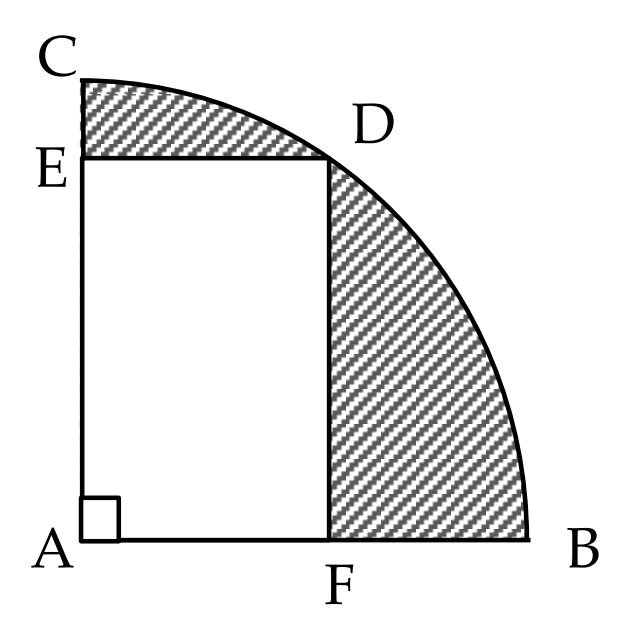
\includegraphics[scale=0.5]{simulasi1-1}
		\end{figure}
		
		\item Sebuah dadu seimbang enam sisi dilempar sebanyak $n$ kali. Jika rata-rata mata dadu yang keluar adalah $\frac{1}{4}n$, maka median dari seluruh nilai $n$ yang mungkin adalah...
		
		
		\item Jika $a,b$ adalah bilangan real positif yang memenuhi $a^{505}+b^{505}=1$, maka nilai minimum dari $a^{2020}+b^{2020}$ adalah...
		
		\item Diketahui segi delapan beraturan $ABCDEFGH$ yang mempunyai panjang sisi 2 cm. Misalkan $A$ adalah himpunan luas semua segitiga yang titik-titik sudutnya diambil dari delapan titik sudut segi delapan tersebut. Jika jumlah semua anggota $A$ adalah $(a+b\sqrt{2})$ cm$^2$, nilai $a+b$ adalah...
		
		\item Bilangan rasional $x=\frac{a}{b}$ terbesar sedemikian sehingga $\frac{5}{a}+20b < 2020$ merupakan kuadrat sempurna untuk suatu bilangan asli $a,b$ adalah...
		
		\item Pada suatu kotak terdapat 40 bola merah dan hijau. Dua bola diambil secara acak dan diamati warnanya. Jika peluang terambil kedua bola berwarna merah adalah $\frac{5}{12}$, maka banyaknya bola merah di dalam kotak semula adalah...
		
		\item Carilah seluruh pasangan bilangan bulat positif $(a,b,x)$ yang memenuhi $x^a+x^b=x^{a+b}$. 
		
		\item Carilah bentuk paling sederhana dari $\sqrt{104\sqrt{6}+468\sqrt{10}+144\sqrt{15}+2006}$.
		
		\item Untuk bilangan real positif $a,b,c$ yang memenuhi $$\frac{a}{a+1}+\frac{b}{b+1}+\frac{c}{c+1} = 1,$$ tentukan nilai maksimum dari $abc$.
		
		\item Azura sedang berada di toko ikan hias dan berniat membeli sepasang ikan koi. Penjaga toko membebaskan Azura untuk mengambil sepasang ikan tersebut dari suatu akuarium besar di tengah toko yang berisi $n>1$ ikan secara acak. Peluang Azura mendapatkan ikan dengan jenis kelamin yang sama adalah $\dfrac12$. Jika banyaknya ikan koi jantan sama dengan tiga kali banyak ikan koi betina, nilai minimum $n$ adalah...
		
		\item Carilah seluruh bilangan bulat positif terkecil yang memenuhi $x^2+x+1 \equiv 0 \mod 49$
		
		\item Misalkan suatu lingkaran mempunyai diameter $AB$ dan $P$ sebagai titik di luar lingkaran tersebut. Garis $PQ$ dan $PR$ menyinggung lingkaran di $Q$ dan $R$. Garis $PH$ berpotongan tegak lurus dengan garis $AB$ di $H$ dan $PH$ berpotongan dengan $AR$ di $S$. Jika $\angle QPH = 40^\circ$ dan $\angle QSA = 30^\circ$, tentukan besar $\angle RPS$.
		
		\item Berapa banyak bilangan real $x$ yang memenuhi $\sqrt[4]{x+15} = \sqrt[3]{x}+1$ ?
		
		\item  Terdapat sebuah rapat yang terdiri dari 40 kursi yang dihadiri oleh 16 tamu undangan.
		Untuk menghindari penularan COVID-19, maka setiap tamu undangan harus dibatasi minimal
		dengan 1 kursi. Tentukan banyaknya susunan mereka duduk.

		
		\item Pada ekspresi $$a= \sqrt{2020+\sqrt{2020+\sqrt{2020+\sqrt{2020+...}}}}$$
		bilangan 2020 muncul sebanyak 1442 kali di dalam akar. Tentukan nilai $\left \lceil a \right \rceil$.
		
		\item Misalkan $ABC$ adalah segitiga dengan $AB=9, BC=20,$ dan $CA=16$. Titik $D$ terletak pada segmen $BC$ sehingga $DB=DA$. Garis bagi luar $\angle BAC$ memotong perpanjangan $BC$ di $E$. Misalkan $F$ adalah titik tengah $DE$. Tentukan panjang $FA$.
		
		\item Untuk sebarang bilangan asli $n \ge 2$, misalkan $A_n$ adalah himpunan semua solusi persamaan $$x=\left\lfloor \frac{x}{2}\right \rfloor+\left\lfloor \frac{x}{3}\right \rfloor+\dots+\left\lfloor\frac{x}{n} \right \rfloor.$$
		
		Jika $S = A_2 \cup A_3 \cup A_4 \cup \dots \cup A_n$, tentukan nilai dari elemen terbesar $S$.
		
		\item Misalkan $ABCD$ adalah segiempat tali busur. Diagonal $AC$ dan $BD$ berpotongan di titik $E$. Jika $BD=24$, tentukan nilai minimum dari $\dfrac{1}{AE}+\dfrac{1}{EC}$.
\end{enumerate}
	
	
\end{document}